%%%%%%%%%%%%%%%%%%%%%%%%%%%%%%%%%%%%%%%%%%%%%%%%%%%%%%%%%%%%%%%%%%%%%%%%%%%%%%%

\documentclass[a4paper,10pt]{llncs}

%%%%%%%%%%%%%%%%%%%%%%%%%%%%%%%%%%%%%%%%%%%%%%%%%%%%%%%%%%%%%%%%%%%%%%%%%%%%%%%

\usepackage[utf8x]{inputenc}
\usepackage{amssymb}
\usepackage{amsmath}
\usepackage{amsfonts}
\usepackage{graphicx}
%\usepackage{llncsdoc}
\usepackage[english]{babel}
\usepackage[ruled,vlined,linesnumbered]{algorithm2e}
\usepackage{algorithmic}
\usepackage{float}
\usepackage{todonotes}
\usepackage{subfigure}

\usepackage{tikz}
\usetikzlibrary{matrix, calc, arrows}

%%%%%%%%%%%%%%%%%%%%%%%%%%%%%%%%%%%%%%%%%%%%%%%%%%%%%%%%%%%%%%%%%%%%%%%%%%%%%%%

%%% 
%%% complexity.tex
%%% 

\usepackage{xspace}

%%% ----------------------------------------------------------------------
%%% complexity classes
%%% ----------------------------------------------------------------------

% TIME
\newcommand{\DTIMEX}{{\sf\bf DTIME}}
\newcommand{\DTIMEclass}{\DTIMEX\xspace}
\newcommand{\DTIME}{\DTIMEclass}
% NL class
\newcommand{\NLclassbase}{{\sf\bf NL}}
\newcommand{\NLclass}{\NLclassbase\xspace}
% P class
\newcommand{\Pclassbase}{{\sf\bf P}}
\newcommand{\Pclass}{\Pclassbase\xspace}
% NP class
\newcommand{\NPclassbase}{{\sf\bf NP}}
\newcommand{\NPclass}{\NPclassbase\xspace}
% coNP class
\newcommand{\coNPclassbase}{{\sf\bf coNP}}
\newcommand{\coNPclass}{\coNPclassbase\xspace}
% PSPACE class
\newcommand{\PSPACEclassbase}{{\sf\bf PSPACE}}
\newcommand{\PSPACEclass}{\PSPACEclassbase\xspace}
% MAXSNP class
\newcommand{\MaxSNPclassbase}{{\sf\bf MaxSNP}}
\newcommand{\MaxSNPclass}{\MaxSNPclassbase\xspace}
% MAXNP class
\newcommand{\MaxNPclassbase}{{\sf\bf MaxNP}}
\newcommand{\MaxNPclass}{\MaxNPclassbase\xspace}
% EPTAS class
\newcommand{\EPTASclassbase}{{\sf\bf EPTAS}}
\newcommand{\EPTASclass}{\EPTASclassbase\xspace}
% FPTAS class
\newcommand{\FPTASclassbase}{{\sf\bf FPTAS}}
\newcommand{\FPTASclass}{\FPTASclassbase\xspace}
% PTAS class
\newcommand{\PTASclassbase}{{\sf\bf PTAS}}
\newcommand{\PTASclass}{\PTASclassbase\xspace}
% APX class
\newcommand{\APXclassbase}{{\sf\bf APX}}
\newcommand{\APXclass}{\APXclassbase\xspace}
% log-APX class
\newcommand{\logAPXclassbase}{{\sf\bf log{\tt -}APX}}
\newcommand{\logAPXclass}{\logAPXclassbase\xspace}
% poly-APX class
\newcommand{\polyAPXclassbase}{{\sf\bf poly{\tt -}APX}}
\newcommand{\polyAPXclass}{\polyAPXclassbase\xspace}
% exp-APX class
\newcommand{\expAPXclassbase}{{\sf\bf exp{\tt -}APX}}
\newcommand{\expAPXclass}{\expAPXclassbase\xspace}
% NPO class
\newcommand{\NPOclassbase}{{\sf\bf NPO}}
\newcommand{\NPOclass}{\NPOclassbase\xspace}
% #P class
\newcommand{\sharpPclassbase}{\#{\sf\bf P}}
\newcommand{\sharpPclass}{\sharpPclassbase\xspace}
% FPT class
\newcommand{\FPTclassbase}{{\sf\bf FPT}}
\newcommand{\FPTclass}{\FPTclassbase\xspace}
% W class
\newcommand{\Wclassbase}[1]{{\sf\bf W[#1]}}
\newcommand{\Wclass}[1]{\Wclassbase{#1}\xspace}
% W class
\newcommand{\XPclassbase}{{\sf\bf XP}}
\newcommand{\XPclass}{\XPclassbase\xspace}
% WNL class
\newcommand{\WNLclassbase}{{\sf\bf WNL}}
\newcommand{\WNLclass}{\WNLclassbase\xspace}
% ZPP class
\newcommand{\ZPPclassbase}{{\sf\bf ZPP}}
\newcommand{\ZPPclass}{\ZPPclassbase\xspace}
% NPK class
\newcommand{\NPKclassbase}{{\sf\bf NPK}}
\newcommand{\NPKclass}{\NPKclassbase\xspace}
\newcommand{\NPKandclass}{\text{$\NPKclass_\text{and}$}\xspace}
\newcommand{\NPKzeroandclass}{\text{$\NPKclass^0_\text{and}$}\xspace}
\newcommand{\NPKorclass}{\text{$\NPKclass_\text{or}$}\xspace}
\newcommand{\NPKzeroorclass}{\text{$\NPKclass^0_\text{or}$}\xspace}

%%% ----------------------------------------------------------------------
%%% complete
%%% ----------------------------------------------------------------------

% keyword
\newcommand{\complete}{\text{-complete}}
% NL-complete
\newcommand{\NLcomplete}{\NLclassbase\complete\xspace}
\newcommand{\NLC}{\NLcomplete}
% P-complete
\newcommand{\Pcomplete}{\Pclassbase\complete\xspace}
\newcommand{\PC}{\Pcomplete}
% NP-complete
\newcommand{\NPcomplete}{\NPclassbase\complete\xspace}
\newcommand{\NPC}{\NPcomplete}
% coNP-complete
\newcommand{\coNPcomplete}{\coNPclassbase\complete\xspace}
\newcommand{\coNPC}{\coNPcomplete}
% PSPACE-complete
\newcommand{\PSPACEcomplete}{\PSPACEclassbase\complete\xspace}
\newcommand{\PSPACEC}{\PSPACEcomplete}
% MAXSNP-complete
\newcommand{\MaxSNPcomplete}{\MaxSNPclassbase\complete\xspace}
\newcommand{\MaxSNPC}{\MaxSNPcomplete}
% APX-complete
\newcommand{\APXcomplete}{\APXclassbase\complete\xspace}
\newcommand{\APXC}{\APXcomplete}
% #P-complete
\newcommand{\sharpPcomplete}{\sharpPclassbase\complete\xspace}
\newcommand{\sharpPC}{\sharpPcomplete}
% W[i]-complete
\newcommand{\Wcomplete}[1]{\Wclassbase{#1}\complete\xspace}
\newcommand{\WC}[1]{\Wcomplete{#1}}
% WNL-complete
\newcommand{\WNLcomplete}{\WNLclassbase\complete\xspace}
\newcommand{\WNLC}{\WNLcomplete}

%%% ----------------------------------------------------------------------
%%% hard
%%% ----------------------------------------------------------------------

% keyword
\newcommand{\hard}{\text{-hard}}
% NL-hard
\newcommand{\NLhard}{\NLclassbase\hard\xspace}
\newcommand{\NLH}{\NLhard}
% P-hard
\newcommand{\Phard}{\NPclassbase\hard\xspace}
\newcommand{\PH}{\Phard}
% NP-hard
\newcommand{\NPhard}{\NPclassbase\hard\xspace}
\newcommand{\NPH}{\NPhard}
% coNP-hard
\newcommand{\coNPhard}{\coNPclassbase\hard\xspace}
\newcommand{\coNPH}{\coNPhard}
% PSPACE-hard
\newcommand{\PSPACEhard}{\PSPACEclassbase\hard\xspace}
\newcommand{\PSPACEH}{\PSPACEhard}
% MAXSNP-hard
\newcommand{\MaxSNPhard}{\MaxSNPclassbase\hard\xspace}
\newcommand{\MaxSNPH}{\MaxSNPhard}
% APX-hard
\newcommand{\APXhard}{\APXclassbase\hard\xspace}
\newcommand{\APXH}{\APXhard}
% WNL-hard
\newcommand{\WNLhard}{\WNLclassbase\hard\xspace}
\newcommand{\WNLH}{\WNLhard}
% #P-hard
\newcommand{\sharpPhard}{\sharpPclassbase\hard\xspace}
\newcommand{\sharpPH}{\sharpPhard}
% W[i]-hard
\newcommand{\Whard}[1]{\Wclassbase{#1}\hard\xspace}
\newcommand{\WH}[1]{\Whard{#1}}

%%% ----------------------------------------------------------------------
%%% hardness
%%% ----------------------------------------------------------------------

% keyword
\newcommand{\hardness}{\text{-hardness}}
% NP-hardness
\newcommand{\NPhardness}{\NPclassbase\hardness\xspace}
% APX-hardness
\newcommand{\APXhardness}{\APXclassbase\hardness\xspace}
% W[i]-hardness
\newcommand{\Whardness}[1]{\Wclassbase{#1}\hardness\xspace}
% WNL-hardness
\newcommand{\WNLhardness}{\WNLclassbase\hardness\xspace}

%%% ----------------------------------------------------------------------
%%% completeness
%%% ----------------------------------------------------------------------

% keyword
\newcommand{\completeness}{\text{-completeness}}
% NL-completeness
\newcommand{\NLcompleteness}{\NLclassbase\completeness\xspace}
% P-completeness
\newcommand{\Pcompleteness}{\NPclassbase\completeness\xspace}
% NP-completeness
\newcommand{\NPcompleteness}{\NPclassbase\completeness\xspace}
% APX-completeness
\newcommand{\APXcompleteness}{\APXclassbase\completeness\xspace}
% #P-completeness
\newcommand{\sharpPcompleteness}{\sharpPclassbase\completeness\xspace}
% W[i]-hard
\newcommand{\Wcompleteness}[1]{\W{#1}-\completeness\xspace}

%%% ----------------------------------------------------------------------
%%% reduction
%%% ----------------------------------------------------------------------

\newcommand{\reduction}{reduction}
\newcommand{\reductions}{reductions}
\newcommand{\reductible}{reductible}

\newcommand{\APTypeReduction}{AP}
\newcommand{\PTASTypeReduction}{PTAS}
\newcommand{\LTypeReduction}{L}
\newcommand{\ETypeReduction}{E}
\newcommand{\fptTypeReduction}{fpt}
\newcommand{\pptTypeReduction}{ptp}

% AP-reduction
\newcommand{\APreduction}{\APTypeReduction-\reduction\xspace}
\newcommand{\APreductions}{\APTypeReduction-\reductions\xspace}
\newcommand{\APreductible}{\APTypeReduction-\reductible\xspace}

% PTAS-reduction
\newcommand{\PTASeduction}{\PTASTypeReduction-\reduction\xspace}
\newcommand{\PTASreductions}{\PTASTypeReduction-\reductions\xspace}
\newcommand{\PTASreductible}{\PTASTypeReduction-\reductible\xspace}

% L-reduction
\newcommand{\Lreduction}{\LTypeReduction-\reduction\xspace}
\newcommand{\Lreductions}{\LTypeReduction-\reductions\xspace}
\newcommand{\Lreductible}{\LTypeReduction-\reductible\xspace}

% E-reduction
\newcommand{\Ereduction}{\ETypeReduction-\reduction\xspace}
\newcommand{\Ereductions}{\ETypeReduction-\reductions\xspace}
\newcommand{\Ereductible}{\ETypeReduction-\reductible\xspace}

% fpt-reduction
\newcommand{\fptreduction}{\fptTypeReduction-\reduction\xspace}
\newcommand{\fptreductions}{\fptTypeReduction-\reductions\xspace}
\newcommand{\fptreductible}{\fptTypeReduction-\reductible\xspace}

% ptp-reduction
\newcommand{\ptpreduction}{\ptpTypeReduction-\reduction\xspace}
\newcommand{\ptpreductions}{\ptpTypeReduction-\reductions\xspace}
\newcommand{\ptpreductible}{\ptpTypeReduction-\reductible\xspace}

% symbols
\DeclareMathOperator{\APreduce}{\text{$\leq_{\text{\APTypeReduction}}$}}
\DeclareMathOperator{\PTASreduce}{\text{$\leq_{\text{\PTASTypeReduction}}$}}
\DeclareMathOperator{\Lreduce}{\text{$\leq_{\text{\LTypeReduction}}$}}
\DeclareMathOperator{\Ereduce}{\text{$\leq_{\text{\ETypeReduction}}$}}
\DeclareMathOperator{\fptreduce}{\text{$\leq_{\text{\fptTypeReduction}}$}}
\DeclareMathOperator{\ptpreduce}{\text{$\leq_{\text{\fptTypeReduction}}$}}

%% 
%% Approximation
%%
\DeclareMathOperator{\poly}{poly}
\DeclareMathOperator{\POLY}{poly}
\DeclareMathOperator{\SIZE}{size}
\newcommand{\sol}{{\sf sol}\xspace}
\newcommand{\PB}[1]{\textsf{\scshape{#1}}}
\newcommand{\OPTname}{opt}
\newcommand{\OPT}{\text{$\mathsf{\bf \OPTname}$}}
\newcommand{\OPTpb}[1]{\text{$\mathsf{\OPTname}_{\PB{#1}}$}}
\newcommand{\ALGO}[1]{\textbf{\ttfamily\sf #1}}
\newcommand{\Approxname}{Approx}
\newcommand{\APPROX}[1]{\text{$\ALGO{\Approxname}_{\,\PB{#1}}$}}
\newcommand{\PCP}{{\sf\bf PCP}\xspace}

%%
%% Problem Definition
%%
\newcommand{\PbDef}[3]{%
\begin{center}
  \begin{tabular}{l}%
    \shadowbox{%
    \begin{minipage}[c]{.9\textwidth}
      \smallskip%
      \par\noindent%
      {#1}%
      \smallskip
      \par\noindent%
      $\bullet$
      \textbf{\textsf{Input}}~: #2% 
      \medskip
      \par\noindent%
      $\bullet$
      \textbf{\textsf{Question}}~:
      #3% 
      \smallskip%
      \par\noindent%
    \end{minipage}
  }% end shadowbox
  \end{tabular}%
\end{center}
}%
\newcommand{\PbDefinition}{\PbDef}

%%
%% Problem (Input + Output) Definition
%%
\newcommand{\PbInputOutputDef}[3]{%
\begin{center}
  \begin{tabular}{l}%
    \shadowbox{%
    \begin{minipage}[c]{.9\textwidth}
      \smallskip%
      \par\noindent%
      \PB{#1}%
      \medskip%
      \par\noindent%
      $\bullet$
      \textbf{\textsf{Input}}~: #2% 
      \medskip
      \par\noindent%
      $\bullet$
      \textbf{\textsf{Output}}~:
      #3% 
      \smallskip%
      \par\noindent%
    \end{minipage}
  }% end shadowbox
  \end{tabular}%
\end{center}
}%
\newcommand{\PbInputOutputDefinition}{\PbInputOutputDef}


%%
%% Optimization Problem Definition
%%

\newcommand{\OptPbDefinition}[4]{%
\begin{center}
  \begin{tabular}{l}%
    \shadowbox{%
    \begin{minipage}[c]{.9\textwidth}
      \par\noindent%
      \shadowbox{#1}%
      \par\noindent%
      $\bullet$
      \textbf{\textsf{Input}}~: #2% 
      \par\noindent%
      $\bullet$
      \textbf{\textsf{Solution}}~: #3%  
      \par\noindent%
      $\bullet$
      \textbf{\textsf{Measure}}~: #4% 
      \par\noindent%
    \end{minipage}
    }% end shadowbox
  \end{tabular}%
\end{center}
}%

%%
%% Parameterized Problem Definition
%%
\newcommand{\ParamPbDefinition}[4]{%
\begin{center}
  \begin{tabular}{l}%
    %\shadowbox{%
    \begin{minipage}[c]{.95\textwidth}
      % \smallskip%
      \par\noindent%
      #1%
      % \smallskip%
      \par\noindent%
      \textbf{\textsf{Input}}~: #2% 
      % \smallskip
      \par\noindent%
      \textbf{\textsf{Question}}~: #3%  
      % \smallskip
      \par\noindent%
      \textbf{\textsf{Parameter}}~: #4% 
      %\smallskip%
      \par\noindent%
    \end{minipage}
  %}% end shadowbox
  \end{tabular}%
\end{center}
}%
\newcommand{\ParamPbDefinitionTwo}[5]{%
\begin{center}
  \begin{tabular}{l}%
    \shadowbox{%
    \begin{minipage}[c]{.9\textwidth}
      \smallskip%
      \par\noindent%
      \shadowbox{#1}%
      \medskip%
      \par\noindent%
      $\bullet$
      \textbf{\textsf{Input}}~: #2% 
%      \medskip
      \par\noindent%
      $\bullet$
      \textbf{\textsf{Parameter}}~: #3% 
 %     \medskip
      \par\noindent%
      $\bullet$
      \textbf{\textsf{Parameter}}~: #4% 
      \medskip
      \par\noindent%
      $\bullet$
      \textbf{\textsf{Question}}~: #5%  
      \smallskip%
      \par\noindent%
    \end{minipage}
    }% end shadowbox
  \end{tabular}%
\end{center}
}%
\newcommand{\ParamPbDefinitionThree}[6]{%
\begin{center}
  \begin{tabular}{l}%
    \shadowbox{%
    \begin{minipage}[c]{.9\textwidth}
      \smallskip%
      \par\noindent%
      \shadowbox{#1}%
      \medskip%
      \par\noindent%
      $\bullet$
      \textbf{\textsf{Input}}~: #2% 
%      \medskip
      \par\noindent%
      $\bullet$
      \textbf{\textsf{Parameter}}~: #3% 
%      \medskip
      \par\noindent%
      $\bullet$
      \textbf{\textsf{Parameter}}~: #4% 
%      \medskip
      \par\noindent%
      $\bullet$
      \textbf{\textsf{Parameter}}~: #5%  
      \medskip
      \par\noindent%
      $\bullet$
      \textbf{\textsf{Question}}~: #6%  
      \smallskip%
      \par\noindent%
    \end{minipage}
    }% end shadowbox
  \end{tabular}%
\end{center}
}%
\newcommand{\ParamPbDefinitionFour}[7]{%
\begin{center}
  \begin{tabular}{l}%
    \shadowbox{%
    \begin{minipage}[c]{.9\textwidth}
      \smallskip%
      \par\noindent%
      \shadowbox{#1}%
      \medskip%
      \par\noindent%
      $\bullet$
      \textbf{\textsf{Input}}~: #2% 
%      \medskip
      \par\noindent%
      $\bullet$
      \textbf{\textsf{Parameter}}~: #3% 
%      \medskip
      \par\noindent%
      $\bullet$
      \textbf{\textsf{Parameter}}~: #4% 
%      \medskip
      \par\noindent%
      $\bullet$
      \textbf{\textsf{Parameter}}~: #5%  
%      \medskip
      \par\noindent%
    $\bullet$
      \textbf{\textsf{Parameter}}~: #6%  
      \medskip
      \par\noindent%
      $\bullet$
      \textbf{\textsf{Question}}~: #7%  
      \smallskip%
      \par\noindent%
    \end{minipage}
    }% end shadowbox
  \end{tabular}%
\end{center}
}%
\newcommand{\ParamPbDefinitionFive}[8]{%
\begin{center}
  \begin{tabular}{l}%
    \shadowbox{%
    \begin{minipage}[c]{.9\textwidth}
      \smallskip%
      \par\noindent%
      \shadowbox{#1}%
      \medskip%
      \par\noindent%
      $\bullet$
      \textbf{\textsf{Input}}~: #2% 
%      \medskip
      \par\noindent%
      $\bullet$
      \textbf{\textsf{Parameter}}~: #3% 
%      \medskip
      \par\noindent%
      $\bullet$
      \textbf{\textsf{Parameter}}~: #4% 
%      \medskip
      \par\noindent%
      $\bullet$
      \textbf{\textsf{Parameter}}~: #5%  
%      \medskip
      \par\noindent%
    $\bullet$
      \textbf{\textsf{Parameter}}~: #6%  
%      \medskip
      \par\noindent%
    $\bullet$
      \textbf{\textsf{Parameter}}~: #7%  
      \medskip
      \par\noindent%
      $\bullet$
      \textbf{\textsf{Question}}~: #8%  
      \smallskip%
      \par\noindent%
    \end{minipage}
    }% end shadowbox
  \end{tabular}%
\end{center}
}%
\newcommand{\ParamPbDefinitionSix}[9]{%
\begin{center}
  \begin{tabular}{l}%
    \shadowbox{%
    \begin{minipage}[c]{.9\textwidth}
      \smallskip%
      \par\noindent%
      \shadowbox{#1}%
      \medskip%
      \par\noindent%
      $\bullet$
      \textbf{\textsf{Input}}~: #2% 
%      \medskip
      \par\noindent%
      $\bullet$
      \textbf{\textsf{Parameter}}~: #3% 
%      \medskip
      \par\noindent%
      $\bullet$
      \textbf{\textsf{Parameter}}~: #4% 
%      \medskip
      \par\noindent%
      $\bullet$
      \textbf{\textsf{Parameter}}~: #5%  
%      \medskip
      \par\noindent%
      $\bullet$
      \textbf{\textsf{Parameter}}~: #6%  
%      \medskip
      \par\noindent%
      $\bullet$
      \textbf{\textsf{Parameter}}~: #7%  
%      \medskip
      \par\noindent%
      $\bullet$
      \textbf{\textsf{Parameter}}~: #8%  
      \medskip
      \par\noindent%
      $\bullet$
      \textbf{\textsf{Question}}~: #9%  
      \smallskip%
      \par\noindent%
    \end{minipage}
    }% end shadowbox
  \end{tabular}%
\end{center}
}%




%%%%%%%%%%%%%%%%%%%%%%%%%%%%%%%%%%%%%%%%%%%%%%%%%%%%%%%%%%%%%%%%%%%%%%%%%%%%%%%

% \renewcommand{\floatpagefraction}{.9}
% \renewcommand{\textfraction}{.1}

%%%%%%%%%%%%%%%%%%%%%%%%%%%%%%%%%%%%%%%%%%%%%%%%%%%%%%%%%%%%%%%%%%%%%%%%%%%%%%%

\DeclareMathOperator{\LEFT}{\ell}
\DeclareMathOperator{\RIGHT}{r}

%%%%%%%%%%%%%%%%%%%%%%%%%%%%%%%%%%%%%%%%%%%%%%%%%%%%%%%%%%%%%%%%%%%%%%%%%%%%%%%

\newtheorem{fact}{Fact}

%%%%%%%%%%%%%%%%%%%%%%%%%%%%%%%%%%%%%%%%%%%%%%%%%%%%%%%%%%%%%%%%%%%%%%%%%%%%%%%

\makeatletter
\newcommand{\pushright}[1]{\ifmeasuring@#1\else\omit\hfill$\displaystyle#1$\fi\ignorespaces}
\newcommand{\pushleft}[1]{\ifmeasuring@#1\else\omit$\displaystyle#1$\hfill\fi\ignorespaces}
\makeatother

%%%%%%%%%%%%%%%%%%%%%%%%%%%%%%%%%%%%%%%%%%%%%%%%%%%%%%%%%%%%%%%%%%%%%%%%%%%%%%%

\begin{document}

%%%%%%%%%%%%%%%%%%%%%%%%%%%%%%%%%%%%%%%%%%%%%%%%%%%%%%%%%%%%%%%%%%%%%%%%%%%%%%%

\title{%
Unshuffling Permutations}%

\author{%
  Samuele Giraudo \and
  St\'ephane Vialette
}% end author
\institute{%
  Universit\'e Paris-Est, LIGM (UMR 8049), CNRS, UPEM, ESIEE Paris, ENPC,
  F-77454, Marne-la-Vallée, France\\
  \email{samuele.giraudo@univ-mlv.fr} \\
  \email{vialette@univ-mlv.fr}
}% end institute
\date{\today}

\maketitle

%%%%%%%%%%%%%%%%%%%%%%%%%%%%%%%%%%%%%%%%%%%%%%%%%%%%%%%%%%%%%%%%%%%%%%%%%%%%%%%

\begin{abstract}
bla bla bla \ldots
\end{abstract}

%%%%%%%%%%%%%%%%%%%%%%%%%%%%%%%%%%%%%%%%%%%%%%%%%%%%%%%%%%%%%%%%%%%%%%%%%%%%%%%

%%
%%
%% ---- Introduction ----
%%
\section{Introduction}
\label{section:Introduction}


%%%%%%%%%%%%%%%%%%%%%%%%%%%%%%%%%%%%%%%%%%%%%%%%%%%%%%%%%%%%%%%%%%%%%%%%%%%%%%%

%%
%% ---- Notations ----
%%
\section{Notations}
\label{section:Notations}


%%%%%%%%%%%%%%%%%%%%%%%%%%%%%%%%%%%%%%%%%%%%%%%%%%%%%%%%%%%%%%%%%%%%%%%%%%%%%%%

%%
%% ---- Algorithmic issues ----
%%
\section{Algorithmic issues}
\label{section:Algorithmic issues}


\begin{proposition}
  \label{proposition:matching}
  Let $\pi \in S_{2n}$.
  Then,
  $\pi$ is the union of two order-isomorphic patterns
  if and only if
  there exists a perfect containment-free mathing
  $\mathcal{M}$ of $G_\pi$ such that
  $\LEFT(\mathcal{M}) \simeq \RIGHT(\mathcal{M})$.
\end{proposition}

\begin{proposition}
  \label{proposition:hardness}
  Deciding whether a permutation is the union of two
  order-isomorphic patterns is \NPC.
\end{proposition}

\begin{figure}[t!]
  \centering
  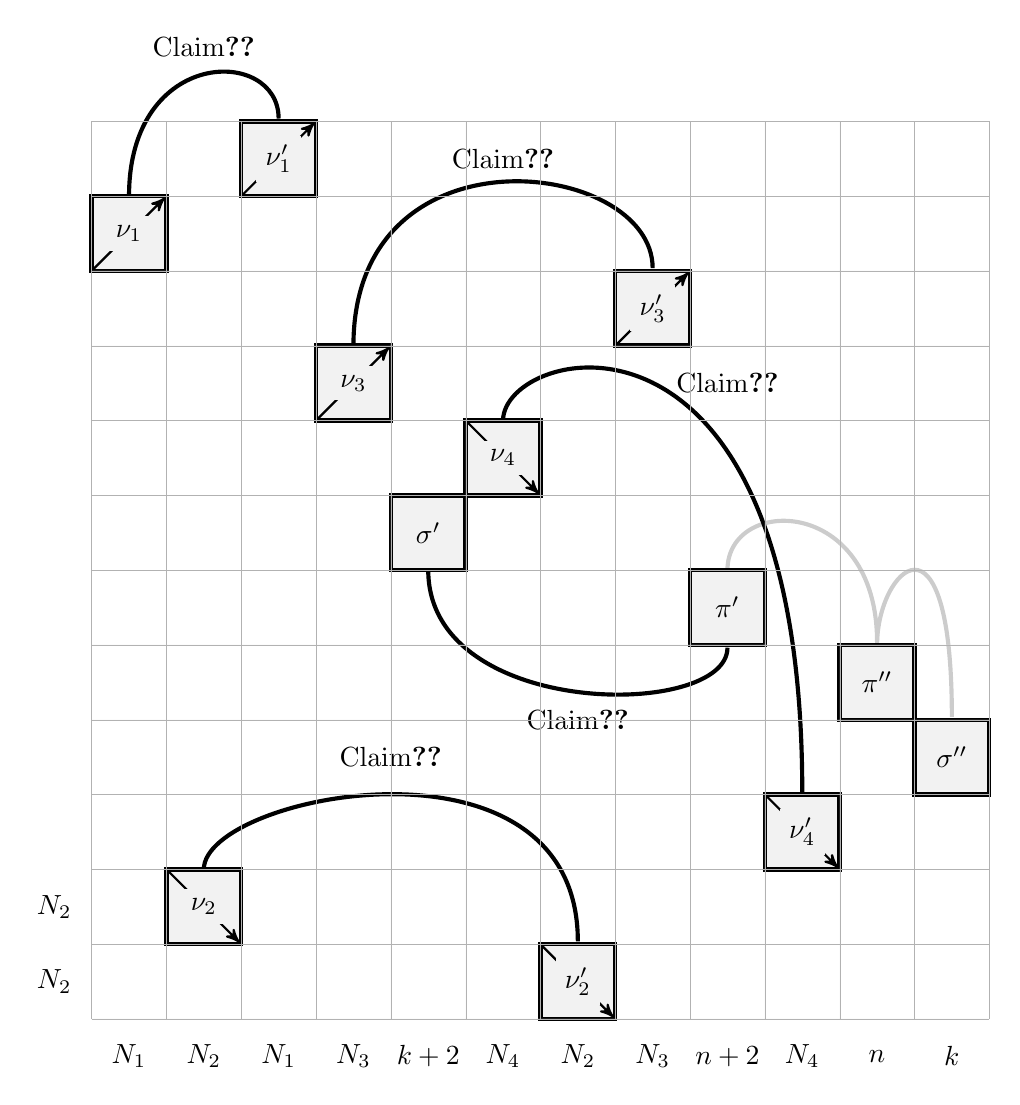
\begin{tikzpicture}[
    scale=.95,
    >=stealth',
    shorten >=1pt,
    main node/.style={align=center},
    cell/.style={draw,ultra thick,fill=black!5},
    structure link/.style={line width=1.5pt},
    pattern link/.style={line width=1.5pt,black!20},
    monotone/.style={->,thick}
    ]  
    % edges
    % pi 1 - pi 2
    \draw [pattern link] (8.5,6) .. controls +(0,1) and +(0,2) .. (10.5,5);
    % pi 2 - sigma 2
    \draw [pattern link] (10.5,5) .. controls +(0,1) and +(0,3) .. (11.5,4);
    % 1
    \draw [structure link] (0.5,11) .. controls +(0,2) and +(0,1) .. (2.5,12);
    \node (claim edge 1) at (1.5,13) {Claim\ref{}};
    % 2
    \draw [structure link] (1.5,2) .. controls +(0,1) and +(0,3) .. (6.5,1);
    \node (claim edge 1) at (4,3.5) {Claim\ref{}};
    % 3
    \draw [structure link] (3.5,9) .. controls +(0,3) and +(0,1.5) .. (7.5,10);
    \node (claim edge 1) at (5.5,11.5) {Claim\ref{}};
    % 4
    \draw [structure link] (5.5,8) .. controls +(0,1) and +(0,7) .. (9.5,3);
    \node (claim edge 1) at (8.5,8.5) {Claim\ref{}};
    % sigma 1 - pi 1
    \draw [structure link] (4.5,6) .. controls +(0,-2) and +(0,-1) .. (8.5,5);
    \node (claim edge 1) at (6.5,4) {Claim\ref{}};
    % nodes
    % 1
    \draw [cell] (0,10) -- (1,10) -- (1,11) -- (0,11) -- cycle;
    \draw [monotone] (0,10) -- ++(1,1) node [midway,fill=white,fill=black!5] {$\nu_1$};
    %\draw [draw,ultra thick,fill=black!5] (0,10) -- (1,10) -- (1,11) -- (0,11) -- cycle;
    \draw [cell] (2,11) -- (3,11) -- (3,12) -- (2,12) -- cycle;
    \draw [monotone] (2,11) -- ++(1,1) node [midway,fill=white,fill=black!5] {$\nu'_1$};
    % 2
    \draw [cell] (1,1) -- (2,1) -- (2,2) -- (1,2) -- cycle;
    \draw [monotone] (1,2) -- ++(1,-1) node [midway,fill=white,fill=black!5] {$\nu_2$};
    \draw [cell] (6,0) -- (7,0) -- (7,1) -- (6,1) -- cycle;
    \draw [monotone] (6,1) -- ++(1,-1) node [midway,fill=white,fill=black!5] {$\nu'_2$};
    % 3
    \draw [cell] (3,8) -- (4,8) -- (4,9) -- (3,9) -- cycle;
    \draw [monotone] (3,8) -- ++(1,1) node [midway,fill=white,fill=black!5] {$\nu_3$};
    \draw [cell] (7,9) -- (8,9) -- (8,10) -- (7,10) -- cycle;
    \draw [monotone] (7,9) -- ++(1,1) node [midway,fill=white,fill=black!5] {$\nu'_3$};
    % 4
    \draw [cell] (5,7) -- (6,7) -- (6,8) -- (5,8) -- cycle;
    \draw [monotone] (5,8) -- ++(1,-1) node [midway,fill=white,fill=black!5] {$\nu_4$};
    \draw [cell] (9,2) -- (10,2) -- (10,3) -- (9,3) -- cycle;
    \draw [monotone] (9,3) -- ++(1,-1) node [midway,fill=white,fill=black!5] {$\nu'_4$};
    % sigma 1
    \draw [cell] (4,6) -- (5,6) -- (5,7) -- (4,7) -- cycle;
    \node [main node] (sigma1) at (4.5,6.5) {$\sigma'$};
    % pi 1
    \draw [cell] (8,5) -- (9,5) -- (9,6) -- (8,6) -- cycle;
    \node [main node] (pi1) at (8.5,5.5) {$\pi'$};    
    % pi 2
    \draw [cell] (10,4) -- (11,4) -- (11,5) -- (10,5) -- cycle;
    \node [main node] (sigma2) at (10.5,4.5) {$\pi''$};
    % sigma 2
    \draw [cell] (11,3) -- (12,3) -- (12,4) -- (11,4) -- cycle;
    \node [main node] (pi2) at (11.5,3.5) {$\sigma''$};  
    % grid
    \draw[step=1cm,black!30,ultra thin,fill=black!10] (0,0) grid (12,12);
    % row size
    \foreach \y/\N in {0.5/N_2,1.5/N_2} {
        \node at (-0.5,\y) (R\y) {$\N$};
    }
    % column size
    \foreach \x/\N in 
    {0.5/N_1,1.5/N_2,2.5/N_1,3.5/N_3,4.5/k+2,5.5/N_4,6.5/N_2,7.5/N_3,8.5/n+2,9.5/N_4,10.5/n,11.5/k} {
        \node at (\x,-0.5) (C\x) {$\N$};
    }
  \end{tikzpicture}
  \caption{\label{fig:reduction}}
\end{figure}


\begin{align*}
N_4 &= 2(2n + k + 2) + 1  = 4n + 2k + 5 \\
N_3 &= 2(2N_4 + 2n + 2k + 4) + 1 = 20n + 12k + 9 \\
N_2 &= 2(2N_3 + 2n + 2k + 4) + 1 \\
N_1 &= 2(2N_2 + 2n + 2k + 4) + 1\text{.}
\end{align*}

\begin{align*}
\sigma'  &= ((k+1) \; \sigma \; (k+2)) \; [2N_2 + N_4 + 2n + k + 2] \\
\pi'     &= ((n+1) \; \pi \; (n+2)) \; [2N_2 + N_4 + n + k + 2] \\
\sigma'' &= \sigma \; [2N_2 + N_4] \\
\pi''    &= \pi \; [2N_2 + N_4 + k] \\
\nu_1    &= \nearrow_{N_1} \; [2N_2 + 2N_3 + 2N_4 + 2n + 2k + 4] \\
\nu'_1   &= \nearrow_{N_1} \; [N_1 + 2N_2 + 2N_3 + 2N_4 + 2n + 2k + 4] \\
\nu_2    &= \nearrow_{N_2} \; [N_2] \\
\nu'_2   &= \searrow_{N_2} \\
\nu_3    &= \nearrow_{N_3} \; [2N_2 + 2N_4 + 2n + 2k + 4] \\
\nu'_3   &= \nearrow_{N_3} \; [2N_2 + N_3 + 2N_4 + 2n + 2k + 4] \\
\nu_4    &= \searrow_{N_4} \; [2N_2 + N_4 + 2n + 2k + 4] \\
\nu'_4   &= \searrow_{N_4} \; [2N_2]
\end{align*}

$$
\mu
=
\nu_1 \; \nu_2 \; \nu'_1 \; \nu_3 \; \sigma' \; \nu_4 \; \nu'_3 \; \pi' \; \nu'_4 \; \pi'' \; \sigma''
$$

\begin{figure}[t!]
  \centering
  \subfigure[A nested $(\nu_1,\nu'_1)$-edge.]{%
    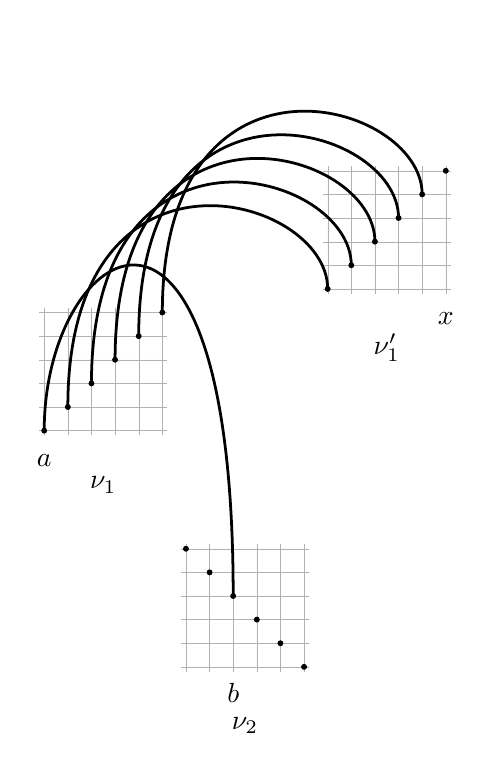
\begin{tikzpicture}
      [
        scale=0.3,
        label/.style={anchor=base}
      ]
      % nu_1
      \draw[step=1cm,black!30,ultra thin,fill=black!10] (-0.2,9.8) grid (5.2,15.2);
      \foreach \x/\y in {0/10,1/11,2/12,3/13,4/14,5/15} {
          \draw [fill=black] (\x,\y) circle (0.1);
      }
      % nu_4
      \draw[step=1cm,black!30,ultra thin,fill=black!10] (5.8,-0.2) grid (11.2,5.2);
      \foreach \x/\y in {6/5,7/4,8/3,9/2,10/1,11/0} {
          \draw [fill=black] (\x,\y) circle (0.1);
      }
      % nu'_1
      \draw[step=1cm,black!30,ultra thin,fill=black!10] (11.8,15.8) grid (17.2,21.2);
      \foreach \x/\y in {12/16,13/17,14/18,15/19,16/20,17/21} {
          \draw [fill=black] (\x,\y) circle (0.1);
      }
      % labels
      \node [label] (x) at (17,14.5) {$x$};
      % \node [label] (y) at (14,14.5) {$y$};
      \node [label] (a) at (0,8.5) {$a$};
      \node [label] (b) at (8,-1.5) {$b$};
      \node (nu1) at (2.5,7.7) {$\nu_1$};
      \node (nu2) at (8.5,-2.5) {$\nu_2$};
      \node (nu1') at (14.5,13.5) {$\nu'_1$};
      % edges
      \draw [line width=1pt]
      (1,11) .. controls +(0,12) and +(0,4) .. (12,16);
      \draw [line width=1pt]
      (2,12) .. controls +(0,12) and +(0,4) .. (13,17);
      \draw [line width=1pt]
      (3,13) .. controls +(0,12) and +(0,4) .. (14,18);
      \draw [line width=1pt]
      (4,14) .. controls +(0,12) and +(0,4) .. (15,19);
      \draw [line width=1pt]
      (5,15) .. controls +(0,12) and +(0,4) .. (16,20);
      \draw [line width=1pt]
      (0,10) .. controls +(0,8) and +(0,20) .. (8,3);
    \end{tikzpicture}
    \label{subfig:no (nu_1, nu_2)-edge - 2}}
  \qquad
  \subfigure[A nested $(\nu_1,\nu'_1)$-edge.]{%
    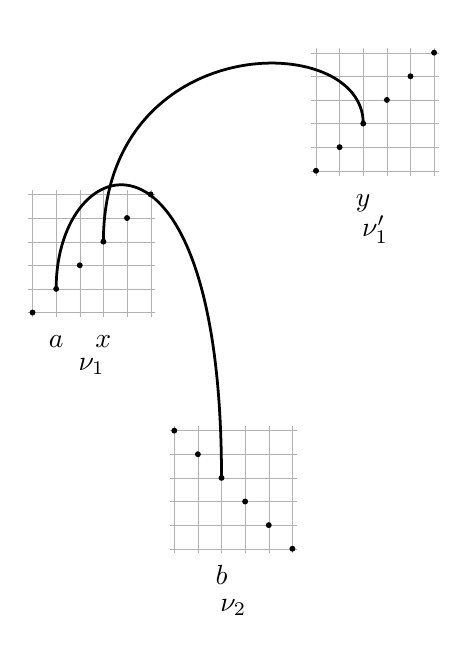
\begin{tikzpicture}
      [
        scale=0.3,
        label/.style={anchor=base}
      ]
      % nu_1
      \draw[step=1cm,black!30,ultra thin,fill=black!10] (-0.2,9.8) grid (5.2,15.2);
      \foreach \x/\y in {0/10,1/11,2/12,3/13,4/14,5/15} {
          \draw [fill=black] (\x,\y) circle (0.1);
      }
      % nu_4
      \draw[step=1cm,black!30,ultra thin,fill=black!10] (5.8,-0.2) grid (11.2,5.2);
      \foreach \x/\y in {6/5,7/4,8/3,9/2,10/1,11/0} {
          \draw [fill=black] (\x,\y) circle (0.1);
      }
      % nu'_1
      \draw[step=1cm,black!30,ultra thin,fill=black!10] (11.8,15.8) grid (17.2,21.2);
      \foreach \x/\y in {12/16,13/17,14/18,15/19,16/20,17/21} {
          \draw [fill=black] (\x,\y) circle (0.1);
      }
      % labels
      \node [label] (x) at (3,8.5) {$x$};
      \node [label] (y) at (14,14.5) {$y$};
      \node [label] (a) at (1,8.5) {$a$};
      \node [label] (b) at (8,-1.5) {$b$};
      \node (nu1) at (2.5,7.7) {$\nu_1$};
      \node (nu2) at (8.5,-2.5) {$\nu_2$};
      \node (nu1') at (14.5,13.5) {$\nu'_1$};
      % edges
      \draw [line width=1pt]
      (3,13) .. controls +(0,9) and +(0,4) .. (14,18);
      \draw [line width=1pt]
      (1,11) .. controls +(0,6) and +(0,16) .. (8,3);
    \end{tikzpicture}
    \label{subfig:no (nu_1, nu_2)-edge - 2}}
    \caption{\label{fig:subfig:no (nu_1, nu_2)-edge}%
            Claim~\ref{claim:no (nu_1, nu_2)-edge}.%
            }
  \end{figure}

\begin{claim}
  \label{claim:no (nu_1, nu_2)-edge}
  There is no $(\nu_1, \nu_2)$-edge in $\mathcal{M}$.
\end{claim}

\begin{proof}[of Claim~\ref{claim:no (nu_1, nu_2)-edge}]
  Suppose, aiming at a contradiction that there exists
  a $(\nu_1, \nu_2)$-edge $e = (a, b)$ in $\mathcal{M}$.
  Without loss of generality, assume $(a, b)$ is the leftmost
  $(\nu_1, \nu_2)$-edge in $\mathcal{M}$.
  \begin{itemize}
  \item $a=1$. 
  Since $\mathcal{M}$ is containment-free, it does
  not contain any $(\nu_1, \nu_1)$-edge.
  Frthermore,
  since $N_1 > 2(2N_2 + 2n + 2k + 4) > 
  |\nu_2| + |\nu'_2| + |\nu_3| + |\nu'_3| + |\nu_4| + |\nu'_4|
  + |\sigma'| + |\pi'| + |\pi''| + |\sigma''|$, there exists 
  a $(\nu_1, \nu'_1)$-edge $e' = (x, y)$ in $\mathcal{M}$.
  We have 
  $\LEFT(e) = \mu(a) < \LEFT(e') = \mu(x)$
  and
  $\RIGHT(e') = \mu(b) < \RIGHT(e') = \mu(y)$
  (see Fig.~\ref{fig:reduction}).
  Therefore, since $\mathcal{M}$ is containment-free, it does
  not contain any $(\nu_2, \nu_2)$-edge.
  According to Proposition~\ref{proposition:matching}, this is 
  a contradiciton.
  \end{itemize}
  \qed
\end{proof}

\begin{fact}
  \label{fact:no (nu_2, nu_2)-edge}
  There is no $(\nu_2, \nu_2)$-edge in $\mathcal{M}$.
\end{fact}

\begin{claim}
  \label{fact:one (nu_1, nu'_1)-edge}
  There is at least one $(\nu_1, \nu'_1)$-edge in $\mathcal{M}$.
\end{claim}

\begin{claim}
  \label{fact:no (nu_2, nu'_1)-edge}
  There is no $(\nu_2, \nu'_1)$-edge in $\mathcal{M}$.
\end{claim}

\begin{claim}
  \label{fact:one (nu_2, nu'_2)-edge}
  There is at least one $(\nu_2, \nu'_2)$-edge in $\mathcal{M}$.
\end{claim}

\begin{fact}
  \label{fact:no (nu'_1, nu'_1),(nu_3, nu_3),(sigma' ,sigma'),(nu_4, nu_4)-edge}
  There is 
  no $(\nu'_1, \nu'_1)$-edge, 
  no $(\nu_3, \nu_3)$-edge,
  no $(\sigma', \sigma')$-edge and
  no $(\nu_4, \nu_4)$-edge
  in $\mathcal{M}$.
\end{fact}

\begin{claim}
  \label{fact:no (nu_3, nu'_2)-edge}
  There is no $(\nu_3, \nu'_2)$-edge in $\mathcal{M}$.
\end{claim}

%%%%%%%%%%%%%%%%%%%%%%%%%%%%%%%%%%%%%%%%%%%%%%%%%%%%%%%%%%%%%%%%%%%%

%%
%% ---- Patterns ----
%%
\section{Patterns}
\label{section:Patterns}

\begin{proposition}
  \label{proposition:patterns:lower bound}
  Let $\pi \in S_{n}$.
  Then $\pi$ contains a pattern of size at least 
  $\left\lfloor\sqrt{n-1}/2\right\rfloor$ that
  is the union of two order-isomorphic patterns.
\end{proposition}

\begin{proof}[of Proposition~\ref{proposition:patterns:lower bound}]
  The Erdös-Szekeres theorem \cite{Erdos:Szekeres:1935} 
  states that every permutation of 
  length at least $pq+1$ must contain either the pattern
  $\nearrow_{p+1}$ or the pattern $\searrow_{q+1}$.
  The result now follows from the fact that
  the pattern $\nearrow_{p+1}$ (resp. $\searrow_{q+1}$)
\qed
\end{proof}

\begin{proposition}
  \label{proposition:patterns:upper bound}
  If $2^{\binom{k}{2}} > \binom{n}{2k}\;\binom{2k}{k}$, then there exists
  a permutation of $S_{n}$ 
  that does not contains a pattern
  of length $2k$ that is the union of two
  order-isomorphic patterns.
\end{proposition}

\begin{proof}[of Proposition~\ref{proposition:patterns:upper bound}]
The proof is by the probabilistic method \cite{Alon:Spencer:1992}.
Let $\pi \in S_n$ be chosen randomly and uniformly.
For any pattern $\sigma$ of length $2k$ ($k$ to be precisely defined latter)
of $\pi$,
let $X_\sigma$ be the indicator variable that 
$\sigma$ is the union of two order-ismorphic patterns.
According to Boole's inequality, we have
$P\left(X_\sigma\right) \leq \binom{2k}{k}\;2^{-k}$.
Since there are $\binom{n}{2k}$ patterns of length $2k$ in $\pi$,
the probability that $\pi$ contains a pattern of length $2k$ 
is the union of two order-ismorphic patterns is at most
$\binom{n}{2k}\;\binom{2k}{k}\;2^{-k} < 1$.
Thus, with positive probability, no event $X_\sigma$ occurs and 
there is a permutation of $S_n$ that does not contain a pattern
of length $2k$ that is the union of two order-isomorphic patterns.
\qed
\end{proof}

%%%%%%%%%%%%%%%%%%%%%%%%%%%%%%%%%%%%%%%%%%%%%%%%%%%%%%%%%%%%%%%%%%%%

%%
%% ---- Conclusion ----
%%
\section{Conclusion}
\label{section:Conclusion}

bla bla blabla bla bla blabla bla bla blabla bla bla blabla bla bla blabla
bla bla blabla bla bla blabla bla bla blabla bla bla blabla bla bla blabla
bla bla blabla bla bla blabla bla bla blabla bla bla blabla bla bla blabla
bla bla blabla bla bla blabla bla bla blabla bla bla blabla bla bla blabla
bla bla blabla bla bla blabla bla bla blabla bla bla blabla.

%%%%%%%%%%%%%%%%%%%%%%%%%%%%%%%%%%%%%%%%%%%%%%%%%%%%%%%%%%%%%%%%%%%%

%%
%% Bibliography
%%

\bibliographystyle{plain}
\bibliography{biblio}

%%%%%%%%%%%%%%%%%%%%%%%%%%%%%%%%%%%%%%%%%%%%%%%%%%%%%%%%%%%%%%%%%%%%%%%%%%%%%%%

\newpage
\section*{Appendix (Reviewers' version only)}

bla bla blabla bla bla blabla bla bla blabla bla bla blabla bla bla blabla
bla bla blabla bla bla blabla bla bla blabla bla bla blabla bla bla blabla
bla bla blabla bla bla blabla bla bla blabla bla bla blabla bla bla blabla
bla bla blabla bla bla blabla bla bla blabla bla bla blabla bla bla blabla
bla bla blabla bla bla blabla bla bla blabla bla bla blabla.

%%%%%%%%%%%%%%%%%%%%%%%%%%%%%%%%%%%%%%%%%%%%%%%%%%%%%%%%%%%%%%%%%%%%%%%%%%%%%%%

\end{document}

%%%%%%%%%%%%%%%%%%%%%%%%%%%%%%%%%%%%%%%%%%%%%%%%%%%%%%%%%%%%%%%%%%%%%%%%%%%%%%%

